\def\difficulty{2}
\sujet{Machine Learning}

\vspace*{10pt}
\begin{note}The objective of this tutorial is to classify images by using machine learning techniques. Some images, as illustrated in Figure \ref{fig:machine_learning:enonce:examples} of the Kimia database will be used \cite{KimiaDB,Sharvit1998}.\end{note}

\begin{figure}[H]
\centering\caption{The different processes will be applied on images from the Kimia database. Here are some examples.}%
\subfloat[bird]{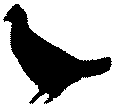
\includegraphics[width=.2\linewidth]{bird-4.png}}
\hfill
\subfloat[camel]{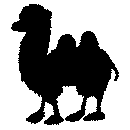
\includegraphics[width=.2\linewidth]{camel-4.png}}
\hfill
\subfloat[ray]{
\includegraphics[width=.2\linewidth]{ray-4.png}}
\hfill
\subfloat[turtle]{
\includegraphics[width=.2\linewidth]{turtle-4.png}}%
\label{fig:machine_learning:enonce:examples}\vspace*{-10pt}%
\end{figure}


\section{Feature extraction}
\index{Characterization}
\index{Features}
The image database used in this tutorial is composed of 18 classes. Each class contains 12 images. All these 216 images come from the Kimia database. In order to classify these images, we first have to extract some features of each binary image. 


\begin{qbox}
\begin{enumerate}
	\item For each image in the database, extract a number of different features, denoted \textsl{nbFeatures}.
	\item Organize these features in an array of \textsl{nbFeatures} lines and 216 columns. In this way, each column $i$ represents the different features of the image $i$.
\end{enumerate}
\end{qbox}

\begin{mcomment}
\begin{mremark}
You can use the Matlab function \minline{regionprops} to extract some features such as area, eccentricity, perimeter, solidity\dots
\end{mremark}
\end{mcomment}

\begin{pcomment}
\begin{premark}
You can use the Python function \pinline{skimage.measure.regionprops} to extract the same geometrical features.
\end{premark}
\end{pcomment}


\section{Image classification}
\index{Classification}
In order to classify the images, we are going to use neural networks. Pattern recognition networks are feedforward networks that can be trained to classify inputs according to target classes.
The inputs are the features of each image. The target data are the labels, indicating the class of each image.

\pagebreak  

\begin{qbox}
\begin{enumerate}
	\item Build the target data, representing the class of each image. The target data for pattern recognition networks should consist of vectors of all zero values except for a 1 in element i, where i is the class they are to represent. In our example, the target data will be an array of 18 lines and 216 columns.
	\item The database will be divided into a training set ($75\%$) and a test set ($25\%$).
	\item Run the training task and classify the test images.
	\item Show the classification confusion matrix as well as the overall performance.
	\item Try to run the same process. What can you conclude?
	\item Try to change the parameters of the network to improve the classification performance.
\end{enumerate}
\end{qbox}

\begin{mcomment}
\begin{mremark}
Look at the Matlab function \minline{patternnet} to make the classification.  Look at the field \textsl{divideParam} of your pattern network for performing the division.
\end{mremark}
\end{mcomment}

\begin{pcomment}
\begin{premark}
Look at the Python module \pinline{sklearn.neural_network.MLPClassifier} to make the classification. Notice that your data may be normalized before performing the classification.
\end{premark}
\end{pcomment}

